\documentclass{beamer}

\usetheme{Madrid}


\usepackage{graphicx} % Allows including images
\graphicspath{{./img/}}

\title{Theia Primer}

\author{Optics Group, Virgo}
\date{Wednesday, May 10\textsuperscript{th} 2017} % Date, can be changed to a custom date

\begin{document}

\begin{frame}
\titlepage % Print the title page as the first slide
\end{frame}


\begin{frame}
\frametitle{Background on astigmatic Gaussian beams}
\begin{columns}
\begin{column}{width=0.45\textwidth}
\begin{itemize}
\item Solutions of the 3D paraxial Helmholtz equation?
\item $ A(\vec x, t) = u(\vec x) e^{ikz} e^{-i\omega t} $

and 

\item $ \nabla_{\bot}^2 u +2ik\frac{\partial u}{\partial z} = 0$$

\end{itemize}
\end{column}

\begin{column}{width=0.45\textwidth}
\begin{itemize}
\item Specify a orthonormal basis $(e_z, e_1, e_2)$: $e_1$ and $e_2$ are principal directions, in which

$$ u(\vec x) =  \mathrm{exp}( i \eta(z) -i\frac{k}{2} (\frac{x^2}{q_x(z)} + \frac{y^2}{q_y(z)}))$$

\item $\Rightarrow$ Orthogonal (simple astigmatic) beam. Ellipsoidal iso-phase surfaces which are \textbf{the same as} the iso-intensity surfaces.
\item Params: $q_x, q_y \in \mathbb{C}$, $(e_1, e_2)$
\end{itemize}
\end{column}

\end{columns}

\end{frame}

%------------------------------------------------

\begin{frame}
\frametitle{Data structures/algorithm/approximations}

\end{frame}

%------------------------------------------------

\begin{frame}
\frametitle{Demonstration}
\begin{itemize}
\item Comparison with \texttt{OptoCAD} for 2D tracing (\texttt{telescope.py})
\item An example in 3D with spherical mirrors (\texttt{sphere.py})
\end{itemize}
\end{frame}


\begin{frame}
\frametitle{Benchmarking: time (i7/8GB)}

\begin{center}
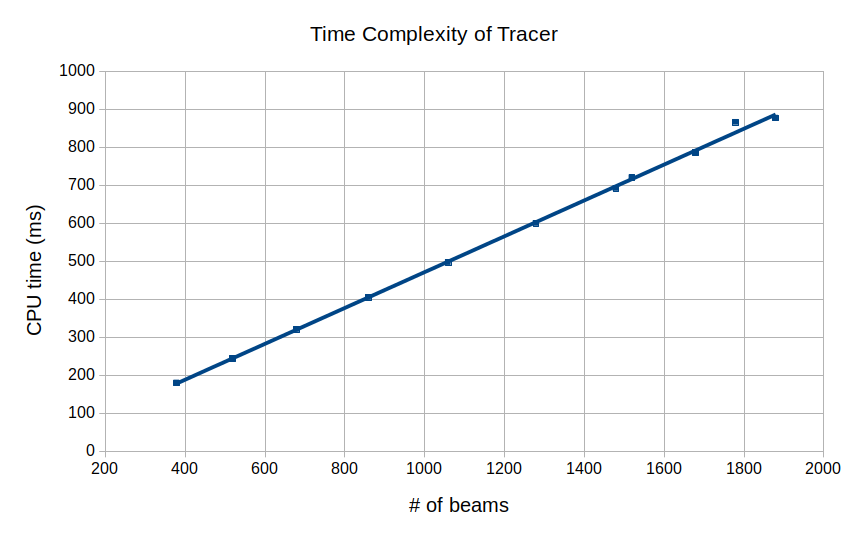
\includegraphics[scale = .45]{timecomplexity.png}
\end{center}


\begin{itemize}
\item CPU = 0.47ms $\times$ (\# beams) ($R^2 = 99.95$\%)
\end{itemize}

\end{frame}

\begin{frame}
\frametitle{Benchmarking: space (i7/8GB)}

\begin{center}
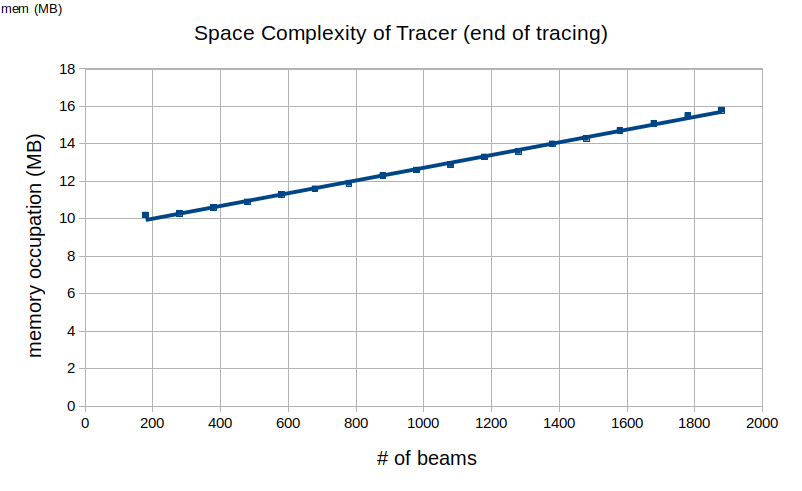
\includegraphics[scale = .45]{spacecomplexity.png}
\end{center}


\begin{itemize}
\item Mem. = 9,3MB + 3,4kB/beam ($R^2 = 99.76$\%)
\end{itemize}
\end{frame}

\begin{frame}
\frametitle{Next steps}

\end{frame}


\begin{frame}

\frametitle{References}

\begin{thebibliography}{99} 

\bibitem{1}
Kochkina, Wanner, Schmelzer, Tr\"obs, Heinzel:
\textit{Modeling of the General Astigmatic Gaussian Beam and its Propagation through 3D Optical Systems},
Applied Optics 24 (2013)

\bibitem{2}
Arnaud, Kogelnik:
\textit{Gaussian Light Beams with General Astigmatism},
Applied Optics 8 (1969)

\end{thebibliography}

\end{frame}


\end{document} 